\documentclass[12pt]{article}

\usepackage{geometry}
\usepackage{amsmath,amssymb,amsthm,epsfig,rotfloat,psfrag,natbib,url,graphicx,lineno}
\usepackage{authblk}
\usepackage{xcolor}
\usepackage{setspace}
\usepackage{mathtools}

\geometry{verbose,letterpaper,tmargin=2.54cm,bmargin=2.54cm,lmargin=2.54cm,rmargin=2.54cm}
\usepackage{caption}
\captionsetup{
  justification = raggedright,
  singlelinecheck = false
}

%%%%
% Some shortcut notation
%%%%
\newcommand{\by}{\ensuremath{\mathbf{y}}}
\newcommand{\bx}{\ensuremath{\mathbf{x}}}
\newcommand{\bz}{\ensuremath{\mathbf{z}}}
\newcommand{\bX}{\ensuremath{\mathbf{X}}}
\newcommand{\bC}{\ensuremath{\mathbf{C}}}
\newcommand{\bW}{\ensuremath{\mathbf{W}}}
\newcommand{\bK}{\ensuremath{\mathbf{K}}}
\newcommand{\bk}{\ensuremath{\mathbf{k}}}
\newcommand{\bI}{\ensuremath{\mathbf{I}}}
\newcommand{\bH}{\ensuremath{\mathbf{H}}}
\newcommand{\bh}{\ensuremath{\mathbf{h}}}
\newcommand{\bw}{\ensuremath{\mathbf{w}}}
\newcommand{\bD}{\ensuremath{\mathbf{D}}}
\newcommand{\bM}{\ensuremath{\mathbf{M}}}
\newcommand{\bR}{\ensuremath{\mathbf{R}}}
\newcommand{\bQ}{\ensuremath{\mathbf{Q}}}
\newcommand{\bu}{\ensuremath{\mathbf{u}}}
\newcommand{\bs}{\ensuremath{\mathbf{s}}}
\newcommand{\bp}{\ensuremath{\mathbf{p}}}
\newcommand{\bP}{\ensuremath{\mathbf{P}}}
\newcommand{\bV}{\ensuremath{\mathbf{V}}}

\newcommand{\bb}{\ensuremath{\boldsymbol{\beta}}}
\newcommand{\bg}{\ensuremath{\boldsymbol{\gamma}}}
\newcommand{\bG}{\ensuremath{\boldsymbol{\Gamma}}}
\newcommand{\ba}{\ensuremath{\boldsymbol{\alpha}}}
\newcommand{\be}{\ensuremath{\boldsymbol{\epsilon}}}
\newcommand{\bSig}{\ensuremath{\boldsymbol{\Sigma}}}
\newcommand{\bmu}{\ensuremath{\boldsymbol{\mu}}}
\newcommand{\bd}{\ensuremath{\boldsymbol{\delta}}}
\newcommand{\bO}{\ensuremath{\boldsymbol{\Omega}}}
\newcommand{\bsig}{\ensuremath{\boldsymbol{\sigma}}}
\newcommand{\bo}{\ensuremath{\boldsymbol{\omega}}}
\newcommand{\bre}{\ensuremath{\boldsymbol{\eta}}}
\newcommand{\bPsi}{\ensuremath{\boldsymbol{\Psi}}}
\newcommand{\btau}{\ensuremath{\boldsymbol{\tau}}}
\newcommand{\bt}{\ensuremath{\boldsymbol{\theta}}}
\newcommand{\bpi}{\ensuremath{\boldsymbol{\pi}}}
\newcommand{\bn}{\ensuremath{\boldsymbol{\eta}}}
\newcommand{\bpsi}{\ensuremath{\boldsymbol{\psi}}}

%mathcal
\newcommand{\fN}{\ensuremath{\mathcal{N}}}
\newcommand{\fG}{\ensuremath{\mathcal{G}}}
\newcommand{\fP}{\ensuremath{\mathcal{P}}}
\newcommand{\fH}{\ensuremath{\mathcal{H}}}
\newcommand{\fS}{\ensuremath{\mathcal{S}}}
\newcommand{\fC}{\ensuremath{\mathcal{C}}}
\newcommand{\fT}{\ensuremath{\mathcal{T}}}

\renewcommand{\thefootnote}{\fnsymbol{footnote}}

\bibliographystyle{apalike}

\raggedright

\begin{document}
\begin{spacing}{1.75}


%\begin{center}
\setlength{\parindent}{0pt}
{\bf Journal}: Ecology 

{\bf Manuscript type}: Statistical Innovation

\bigskip\bigskip
\begin{center}

{\Large \bf Predicting Space-Use with Continuous-Time Markov Chain Movement Models}

\bigskip\bigskip

{Devin S. Johnson}$^{1,*}$, Michaela A. Kratofil$^{2,3}$, Janelle J. Gardner$^1$, Robin W. Baird$^3$, and \\ Amanda L. Bradford$^1$ \bigskip

$^1$Pacific Islands Fisheries Science Center, National Marine Fisheries Service, NOAA, Honolulu, Hawaii, USA 

$^2$Marine Mammal Institute, Department of Fisheries, Wildlife, and Conservation Sciences, Oregon State University, Newport, Oregon, USA

$^3$Cascadia Research Collective, Olympia, Washington, USA

$^*$Corresponding author: {\tt devin.johnson@noaa.gov}


\bigskip

\today

\end{center}

%\vspace*{0.15\textheight}
\vspace*{\fill}

\clearpage


%% ABSTRACT %%%%%%%%%%%%%%%%%%%%%%%%%%%%%%%%%%%%%%%%%%%%%%%%%%%%%
\raggedright
\setlength{\parindent}{2em}
\raggedbottom
\linenumbers


\noindent {\bf Abstract.}
Remote animal telemetry data is widely used in ecology to assess animal space-use and evaluate utilization distributions (UDs). However, traditional empirical UDs (like kernel density or Brownian bridge estimators) can suffer from "start bias" if tag deployments are too short for an animal to fully explore its habitat, heavily biasing results toward the initial release location. Recently, predictive UDs have been proposed in an attempt to mitigate this by finding the long-run stationary distribution of a stochastic process that uses habitat covariates to describe movement. This stationary distribution is free from start bias because it uses habitat variables to predict space-use in the future based on short term movements. Predictive UDs have been calculated from Langevin diffusions as well as general continuous-time Markov chain models (CTMC). While log-linear closed form UD calculations are possible for Langevin models with coefficients directly relating habitat to space-use, CTMC UDs have only been calculated numerically with no parameters directly relating habitat to use. Here we present a general class of CTMC models and show they have a closed form log-linear predictive UD. CTMCs have several benefits over Langevin models: (1) the exact likelihood can be used without approximation, (2) both categorical and continuous habitat variables can be used, and (3) fixed barriers to movement (e.g., land in movement of marine species) are automatically accounted for as part of the model. The R package {\tt walk} was developed for fitting these models in practice and it is used demonstrate explicit UD estimation from CTMC models with a small data set of Hawaiian false killer whales (\emph{Pseudorca crassidens}), including population inference from individual UDs.  


 \bigskip

\noindent {\bf Key words}: CTMC, Hidden Markov model, stationary distribution, Satellite telemetry, Space-use, Utilization distribution

% \clearpage

\section{Introduction}

Any quick literature search will reveal that remote collection and analysis of animal locations, or telemetry data, have become a ubiquitous and important tool in the advancement of animal ecology. A perennial subject within animal telemetry analysis is the assessment of space-use. The topic of animal space-use is often used in conjunction with the terms home range \citep{Burt1943a} or resource selection \citep{Johnson:1980kh}, but here we are specifically concerned with the concept of utilization distributions (UD; \citealt{powell2012home}).  UDs are a spatial probability distribution that describes an animal's location at any random time. As opposed to standard \citep{Keating:2009hl} or correlated kernel density estimates such as Brownian bridge \citep{Horne:2007mw} or AKDE \citep{fleming2015rigorous,calabrese2016ctmm} we consider UD models that explicitly relate habitat variables to use through the log-linear form, 
\begin{equation}
\label{eq:exp.form}
\bu(\bs) \propto \exp\{\bx(\bs)'\bb\},
\end{equation} 
where $\bu(\bs)$ is the UD at location $\bs$ and $\bx(\bs)$ are habitat covariates at location $\bs$. Inference for parametric space-only UDs from temporally correlated telemetry data can be challenging \citep{Johnson:2013fk}. Estimates that ignore the temporal aspect can suffer from start-bias \citep{whitehead2013inferring, calabrese2016ctmm} if the individual does not have a long enough deployment to fully explore its home range. Also, treating locations as independent will underestimate uncertainty in $\bb$ inference \citep{Alston:2023aa}.  

To account for autocorrelated telemetry data predictive UDs have been proposed. Predictive UDs are derived by fitting an autocorrelated movement model to the telemetry data and probability of use id determined from the stationary distribution of the movement model. Predictive UDs can help eliminate start bias because they predict where the individual will be in the long-run \citep{whitehead2013inferring} and the estimated parameters were estimated by explicitly modeling autocorrelation. \cite{Barnett:2008wj} and \cite{moorcroft1999home} considered mechanistic stochastic differential equation (SDE) movement models but the resulting UD was time consuming to numerically assess. This approach was also used to scale step-selection models to the resulting UD \citep{potts2022scale}. Langevin diffusions were proposed as an alternative SDE model because they have a log-linear form (\ref{eq:exp.form}) stationary distribution \citep{michelot2018langevin}. However, only continuously valued habitat variables could be used. Moreover, a 2-stage imputation procedure \citep{ScharfEtAl2017a} is necessary for approximate inference unless the telemetry data is sufficiently fine scale. Also, In study areas with complex barriers to movement, such as coastal marine environments, the imputation approach can become challenging to implement. 

Continuous-time Markov chain (CTMC) movement models have become another type of movement model that can easily incorporate habitat variables to describe movement. We provide a brief description here, but more technical details can be found in \citep{norris1998markov}. In a CTMC movement model the geographical study domain is partitioned into a cells or other discrete locations indexed by $\fC = \{1,\dots,n\}$ (See Figure 1B-E). Each cell, $i$, has a set of neighboring cells $\fN_i = \{j\in \fC: i \sim j\}$, where $i\sim j$ means that an animal can go from cell $i$ to cell $j$ in one move. For example, in a raster partition, neighboring cells might share a border (rook neighborhood) or a corner point(queen neighborhood). CTMC models are defined by the conditional movement rates between cells, $\lambda_{ij} \ge 0$. The total rate of movement away from cell $i$ is $\Lambda_i = \sum_{j\in\fN_i} \lambda_{ij}$. After an individual enters cell $i$ it will reside there an exponential, mean $\Lambda_i^{-1}$, amount of time, then transition to a neighboring cell with probability $P_{ij}=\lambda_{ij}/\Lambda_i$. Two important benefits of CTMC models over SDEs is that categorical habitat variables can be used and CTMCs can be formulated as large sparse hidden Markov models (HMMs) so that efficient evaluation of the exact likelihood is possible. Although to this point most analyses of satellite location telemetry data with CTMCs have also relied on imputation, e.g., \cite{Hanks:2015aa, wilsonestimating, Johnson353516}, but see \cite{pedersen2011estimating} for an archival tag CTMC HMM. One additional benefit of CTMCs relative to SDEs is that complex barriers can be easily accounted for by simply the definition of the cell partitions \citep{wilsonestimating}, that is, for a cell $j$ where the animal cannot travel, $\lambda_{ij}\equiv0$ for all $i \in \fN_j$. Or, in other words $j \notin \fC$. If we put all the rates in an $n \times n$ matrix $\bQ$ with $(-\Lambda_1,\dots,-\Lambda_n)$ on the diagonal and $\lambda_{ij}$ in the $i$th row, $j$th column then one can also represent a CTMC as the discrete-space SDE,
\[
\frac{\text{d}}{\text{d}t}\bu_t = \bQ\bu_t,
\] 
where $\bu_t$ is the distribution of the individuals location at time $t$. The solution to this SDE is,
\[
\bu_t = \bG(t)\bu_0,
\]
where $\bG(t) = \exp(\bQ t)$ is the transition probability matrix (TPM) and here ``$\exp$'' is the matrix exponential function. If the rates and study area are constructed such that: (1) rates are constant through time (homogeneity), (2) any cell can be reached from any other cell given sufficient time (irreducibility), and (3) once a cell is departed the probability of returning in a finite amount of time is $>0$ (positive recurrence), then the CTMC will have a stationary distribution $\bu_t \to \bu$ as $t\to \infty$ \citep{whitehead2013inferring, wilsonestimating}. This stationary distribution is the eigenvector of $\bQ$ associated with the zero eigenvalue. Therefore, a general CTMC movement model does not have the interpretable log-linear form in (\ref{eq:exp.form}) with parameters that directly relate use to habitat variables as it must be numerically determined.  

In order to blend the benefits of the CTMC based movement model with the closed-form, log-linear UD of the Langevin SDE model we propose a class of CTMC models for which one can obtain closed-form log-linear predictions of the UD from the fitted movement model parameters. Markov Chain Monte Carlo (MCMC) theory is used to verify that these specific models possess the desired form for their stationary distributions (e.g., \citealt{michelot2018linking, Blackwell2026a}) and we develop the HMM likelihood for fitting the model, specifically for normally distributed location error. To fit these models, we developed the {\tt R} package {\tt walk}\footnote{Available from: \url{https://dsjohnson.r-universe.dev/walk}} to estimate parameters of general CTMC models using the exact HMM likelihood \citep{mcclintock2020uncovering}. The process of fitting models and making UD inference is demonstrated with telemetry data from a false killer whale (\emph{Pseudorca crassidens}) population in the Hawaiian Islands. 


\section{Explicit Utilization Distribution CTMC Models}

General CTMCs do not have a closed-form stationary distributions but here we propose a class of CTMC useful for animal movement modeling for which we can directly evaluate the stationary distribution. The movement rates of this class have the form, 
\begin{equation}
\label{eq:rate}
\log(\lambda_{ij}) = \bx_{1i}'\ba + \bx_{2j}'\bd + (\bx_{3j}-\bx_{3i})'\bg + \bx_{4ij}'\bn,
\end{equation}
where $\bx_{1i}$ is a set of habitat covariates recorded in the current cell $i$, $\bx_{2j}$ are other covariates recorded in cell $j \in \fN_i$, $\bx_{3j}-\bx_{3i}$ are local differences of a third set of habitat covariates, and $\bx_{4ij}$ are symmetric pair specific covariates ($\bx_{4ij}=\bx_{4ji}$) such as, say, distance between $i$ and $j$. The covariates in $\bx_1$ only control residence time and do not affect which cell an individual might choose upon moving. The variables in $\bx_2$ primarily function to specify preference for neighboring cells based on the absolute value of the covariates, while the variables included via local differences, $\bx_3$, control movement based on relative habitat differences. Both of these movement effects also influence residence time as well. That is if a pull to another habitat is strong a movement to that cell is more likely in the near term. Now that we have a defined class of CTMC movement models we can evaluate the stationary utilization distribution. 

\subsection{Evaluating the stationary utilization distribution}

To evaluate the stationary distribution and make sure one exists we first check the 3 convergence criteria. First, all rates are homogeneous through time. Second, all movement rates in (\ref{eq:rate}) are positive for finite covariates and coefficients, therefore if $i\sim j$, then $j \sim i$. Finally, if the study area is not divided into separate regions for which inter-region moves are impossible, then the positive rates imply irreducibility and positive recurrence. 

We have established that, outside of pathological habitat variables and study areas, a CTMC with rates defined by (\ref{eq:rate}) will have a stationary utilization distribution. To assess what the actual form of the UD is we begin with another theoretical result for evaluating a CTMC stationary distribution, that is,
\begin{equation}
\label{eq:embed.u}
u_i \propto \pi_i / \Lambda_i,
\end{equation}
where $\bpi$ is the stationary distribution of the embedded Markov chain of the CTMC \citep{norris1998markov, wilsonestimating}. The embedded Markov chain is the discrete-time list of cells visited by the CTMC disregarding the actual times when it moves. The embedded Markov chain is an actual discrete-time Markov chain with transition probabilities, $P_{ij}$.  Therefore, we can work in the discrete-time to find the stationary distribution of the CTMC.       
  
One area of probability oriented toward constructing Markov chains which have a specified stationary distribution is Markov Chain Monte Carlo (MCMC). So we can MCMC theoretical results \citep{michelot2018linking,Blackwell2026a} to show that a CTMC movement model has a stationary distribution of log-linear form. To verify the closed-form stationary distribution we need only check that the MCMC reversibility condition is satisfied for a given $\bpi$, that is,
\[
\pi_iP_{ij} = \pi_jP_{ji},
\]
for all $i$ and $j$ in $\fC$ \citep{Blackwell2026a}. By inserting $P_{ij}$ and $P_{ji}$ into the equation, one can check that it is satisfied for $\pi_i \propto \exp(-\bx_{1i}'\alpha + \bx_{2i}'\bd + 2\bx_{3i}'\bg)\Lambda_i$ (See online supplement S1). This implies, using (\ref{eq:embed.u}), the stationary UD for the full CTMC model is, 
\begin{equation}
\label{eq:u.exp}
\begin{aligned}
u_i &\propto \exp(-\bx_{1i}'\ba + \bx_{2i}'\bd + 2\bx_{3i}'\bg)\\
&= \exp(\bx_i'\bb),
\end{aligned}
\end{equation}
where $\bx_i = (\bx_{1i}', \bx_{2i}', \bx_{3i}')'$ and $\bb = (-\ba',\bd', 2\bg')'$. 
  
\subsection{Parameter Estimation}

Previous estimation of CTMC movement parameters using satellite location telemetry data used an imputation method (see \citealt{ScharfEtAl2017a}) which fills in missing cell locations between location acquisition times \citep{Hanks:2015aa, wilsonestimating, Johnson353516}. Even though the imputation method attempts to propagate the uncertainty of the missing locations, it is unclear how this affects estimation of the parameters. Therefore we will use the exact, although potentially more computationally expensive hidden Markov model (HMM) formulation of the model that is often use for CTMC analysis marine fish movement from archival telemetry tags (e.g., see CH. 10 of \citealt{thorson2024spatio}). 

\subsubsection{Satellite telemetry data specification and processing}
For the proposed analysis we consider satellite telemetry data for an individual of the form $\by = \{\by_1,\dots,\by_K\}$, where $\by_k = (\bs_k, t_k, \bpsi_k)$, $\bs_k$ is the observed location of the individual within the study area at time $t_k$ and $\bpsi_k$ represents information or parameters governing location uncertainty. For example, $\bpsi_k$ might represent the major and minor error ellipse lengths of a Kalman Filtered Argos location \citep{mcclintock2015modelling} or a known error radius for GPS locations, e.g., 20m. From these locations we translate the continuous-space data locations and uncertainty to the discrete space, $\fC$, using a function, say, $p(\by_k,\fC) = \bp_k = (p_{1k},\dots,p_{nk})$, where $p_{ik}$ is the probability that the animal is located within cell $i$ at time $t_k$. We used a general form because the function, $p$, will depend on how location uncertain is assessed for the specific satellite and tag hardware. However, uncertainty in the true location, $\bmu_k$, is often represented by the bivariate Normal distribution $\bmu_k \sim N(\bs_k, \bSig_k)$, where $\bpsi_k = \bSig_k$. In that case, $p_{ik}$ would represent the mass of the Normal distribution contained within the $i$th cell. For a raster grid partitioning of the study area this can be calculated by,
\[
p_{ik} = \text{CDF}(x_{i2}, y_{i2}) - \text{CDF}(x_{i2}, y_{i1}) - \text{CDF}(x_{i1}, y_{i2}) + \text{CDF}(x_{i1}, y_{i1})
\]    
where $[x_{i1}, x_{i2}] \times [y_{i1}, y_{i2}]$ is the bounding box for the $i$th cell and $\text{CDF}$ is the bivariate normal cumulative density function with mean $\bs_k$ and covariance $\bSig_k$ (see Figure S1 for illustration of $\bp_k$). A Monte Carlo option for very general error distributions would be to draw a sufficiently large sample from the distribution and assess the proportion of samples that falls within each cell. if the error distribution is known, this only has to be done one time.  

\subsubsection{Likelihood calculation}

For an individual, the likelihood is calculated with the matrix equation \citep{zucchini2016hidden, mcclintock2020uncovering},
\begin{equation}
\label{eq.lik}
[\by|\ba,\bd,\bg,\bn] = \bu_1'\bP(\by_1)\bG(t_2-t_1)\bP(\by_2)\cdots\bG(t_{K}-t_{K-1})\bP(\by_K)\mathbf{1}
\end{equation}
where $\bu_1$ is the location probability distribution at $t_1$, $\bP(\by_k) = \text{diag}(\bp_k)$, $\bG(t_k-t_{k-1})$ is the TPM evaluated over the interval $t_k-t_{k-1}$, and $\mathbf{1}$ is a vector of 1s. The natural choice for $\bu_1$ is $\bu$, the stationary distribution defined by the CTMC movement model, but there are other choices. For example, if a telemetered individual was released at a known location after tagging that may not be representative of its usual movement, then $\bu_1$ would be a vector of all 0s except for the cell containing the release site, which would be a 1. In the false killer whale example below, we use $\bu_1=\bu$ because they were tagged where they were encountered in the wild. In the R package {\tt walk} we use scaling methods to avoid numerical underflow and well as the efficient sparse matrix methods presented in  \cite{sherlock2021direct} to calculate products of the form $\mathbf{v}'\exp\{\bQ(t_k-t_{k-1})\}$.

In addition to the matrix exponential evaluation numerical savings, another optional approach to save computational effort is to set a censoring value for the maximum $\Lambda_i$ value. The numerical methods of \cite{sherlock2021direct} require more matrix operations for higher values of $\max(\Lambda_i)$. For some cells, the log linear $\lambda_{ij}$ model may produce rates of movement that are unrealistically high in some parts of the study area. With respect to UDs this would imply that an individual will not remain in that cell and the $u_i \approx 0$. \cite{Hewitt:2023aa} considered a logit rate model that restricts this behavior, but that model does not allow us to construct a CTMC with an explicit stationary distribution. So, we propose picking a censoring value, say, $\Lambda^*$ and setting $\lambda_{ij}^* = (\Lambda^*/\Lambda_i)\lambda_{ij}$
if $\Lambda_i > \Lambda^*$. If $\Lambda^*$ is sufficiently large, this will have negligible impact on $\bu$ estimation but can dramatically help likelihood computation. One reasonable way to choose $\Lambda^*$ is to select the minimum amount of time that an animal would likely to reside in a cell, say $r^*$. Then set the minimum $\Lambda^* = 1/r^*$. This implies that the expected residency time $\le r^*$. for all cells. The effect on $\bu$ can be verified by comparing the exact, numerically calculated $\bu$ from the censored rate model \citep{wilsonestimating} to $u_i \propto \exp(\bx_i'\bb)$. If discrepancies are sufficiently large, $\Lambda^*$ can be increased. In the resulting model, if $\max(\Lambda_i) \le \Lambda^*$ the UDs are identical. 

Once the CTMC movement model has been fitted the maximum likelihood estimate of $\hat{\bb}_\text{CTMC}= (\ba', \bd', \bg')'$ needs to be transformed to the UD coefficients via $\hat{\bb} = \bM \hat{\bb}_\text{CTMC}$ and $\bM = \text{diag}((-\mathbf{1}_\alpha', \mathbf{1}_\delta', 2\mathbf{1}_\gamma')')$
Thus, the large sample covariance matrix of the UD coefficients is $\hat{\mathbf{S}} = \bM \hat{\mathbf{S}}_\text{CTMC} \bM$, where $\hat{\mathbf{S}}_\text{CTMC}$ is the Hessian-derived large sample covariance matrix of $\hat{\bb}_\text{CTMC}$. If only the standard errors are desired, one can simply multiply the CTMC coefficient standard errors by the multipliers, but if the entire covariance matrix is desired the matrix multiplication is necessary. 

\subsubsection{Population-level inference}

Individual estimates of UD coefficients and predicted UDs can be difficult to interpret for population inference and management considerations. Therefore, we suggest the more appropriate model to fit is the Bayesian random effects model,
\[
\begin{array}{c}
{}[\by_1,\dots,\by_N|\bb_1,\dots,\bb_N] = \prod_{l=1}^N [\by_l|\bM^{-1}\bb_l, \bn_l] \\
{}[\bb_1,\dots,\bb_N|\bt, \bSig] = \prod_{l=1}^N N(\bb_l|\bt, \bSig)
\end{array}
\]
where $\by_l$ is the observed data for individual $l=1,\dots,N$, $\bM^{-1}\bb_l = (\ba_l', \bd_l', \bg_l')'$ and $\bn_l$ are the movement parameters for individual $l$, and the prior distribution for the random population mean coefficient and variance is $[\bt][\bSig]$. Even if individual inference is desired, it is useful to fit this hierarchical model because it allows us to share information between individuals. That is we can make inference to the posterior distribution $[\bb_l|\by_1,\dots,\by_N]$. If we assume that there is some similarity in movement between individuals then we can leverage all data for better individual inference. However, due to the computational demands for fitting the CTMC model to one individual, a full joint random effects model is not currently feasible. 

Even though we cannot fit the full random effects model all at once. We can tailor the general 2-stage meta-analysis methods of \cite{johnson2022greater} to approximate inference for the hierarchical CTMC model using maximum likelihood estimates for each individual. In the first stage individual MLEs, $\hat{\bb_l}$ and covariance matrices, $\hat{\mathbf{S}}_l$ are obtained using (\ref{eq.lik}). In the second stage the MLEs are used as responses in the multivariate linear mixed model,
\[
\hat{\bb}_l = \bt + \bz_l + \be_l; \quad l=1,\dots,N
\]
where the random effect is $[\bz_l|\bSig] = N(\mathbf{0},\bSig)$, the error term is $[\be_l|\hat{\mathbf{S}}_l] = N(\mathbf{0},\hat{\mathbf{S}}_l)$. REML or Laplace approximation procedures are used to fit this model subject to the prior constraint of $[\bt][\bSig]$. Following second stage model fitting we can extract the approximate MAP estimates $\bar{\bt}$ and  $\bar{\bb}_l = \bar{\bt} + \bar{\bz}_l$, where $\bar{\bb}_l$ is the approximate MAP of the posterior $[\bb_l|\by_1,\dots,\by_N]$.


\section{False Killer Whale Space-Use}

In this section, we will apply the modeling approach described in the previous sections to a telemetry dataset on endangered false killer whales (FKW; \emph{Pseudorca crassidens}) in the Hawaiian Islands (\citealt{baird2016lives}). This particular population is resident to the insular waters of the main Hawaiian Islands (MHI; includes Kaua`i/Ni`ihau, Oahu, Maui Nui, and Hawai`i Island) and is comprised of five social clusters, or groups of close family members and regular associates \citep{baird2008false, baird2019cooperative, baird2016lives, martien2019fidelity}. These whales are known to move quickly and frequently among island areas throughout their range \citep{baird2010movements, baird2012range, baird2021bringing, baird2016lives}. Due to inherent challenges associated with tracking apex marine predators, this dataset is characterized by variable deployment durations and irregular location data streams. Considering these factors may drive start bias, as well as their expansive range, we deem this an appropriate dataset to empirically demonstrate the utility of predictive UDs. For the purposes of this assessment, we only focus on movements of 5 individuals that were satellite tagged in 2021 and 2022. There is one representative from each social cluster in the data.   

\subsection{Satellite tag data}

False killer whale satellite tag deployment methods have been described in detail elsewhere (see \citealt{baird2010movements, baird2012range}) so they are only briefly summarized here. Individuals were tagged with Argos transmitting SPOT6 ($n=4$) and SPLASH10 ($n=1$) tags during dedicated small boat survey efforts throughout the main Hawaiian Islands (\citealt{baird2012range,baird2021bringing, baird2016lives}; see \citealt{baird2013odontocete} for details on surveys). Deployment duration for these data ranged from 12 days to 81 days (median=40 days). Argos location data were processed through the Douglas-Argos Filter (accessed via Movebank; \citealt{kranstauber2011movebank,douglas2012moderating}) to remove erroneous locations based on unrealistic travel speeds and turning angles. The final analytical dataset consisted of 5 trajectories and 4,009 filtered Argos and Fastloc GPS (SPASH10 tag) locations (Figure \ref{fig.data}A). For the Argos locations, we used the Kalman-filter diagnostic ellipse data to construct error covariance matrices \citep{mcclintock2015modelling}. While for the Fastloc GPS locations, we used the 95\% quantile error ranges from \cite{dujon2014accuracy}, based on the number of satellites acquired, as twice the standard deviation of the normal error.       

\subsection{Study area and habitat variables}

The official management range of the MHI stock of FKW was documented in \cite{BradfordEtAl2015a} and represents a minimum convex polygon surrounding a buffer of the main Hawaiian Islands (Figure \ref{fig.data}A). This is the study area boundary we use for the UD analysis. 

We used two modeled global oceanographic variables from E.U. Copernicus Marine Service: (1) Sea Surface Temperature (SST; $^\circ$C; DOI: \url{https://doi.org/10.48670/moi-00016}) and (2) Sea Level Anomaly (SLA; m; DOI: \url{https://doi.org/10.48670/moi-00148}) to model movement and space-use. SST is available at $0.082^\circ$ resolution and SLA is available at $0.125^\circ$ degree resolution. In order to match resolution we chose to project the SLA raster to the resolution of the SST raster to avoid loosing oceanographic information. Because we are using these variables to predict long term space-use, we used a single layer for each variable that was the 2 year daily average in the study area. This allowed us to model movement with respect to typical oceanographic conditions (Figure 1B-C). 

In addition to the oceanographic variables, we used distance from land (m) to model FKW's resident nature in the MHI. Also, we also constructed a depth residual variable by using data from the global, 30 arc-second ETOPO elevation model \citep{etopo2022} and removing the linear trend of distance from land. The distance and depth variables were projected to the $0.082^\circ$ SST resolution as well. Then all data, including telemetry data, were projected to the Hawaii Albers Equal Area projection, ESRI:102007 (Figure 1D-E) 

\subsection{CTMC model and population inference \label{sec.fkw.model}}

Notationally, the CTMC movement rate model we used to model the movement of each individual $l=1,\dots,5$ was
\[
\log \lambda_{ij} = \underbrace{\text{(Intercept)} +\text{DEPTH}_i + \text{SST}_i + \text{SST}^2_i + \text{SLA}_i + \text{SLA}^2_i}_{\bx_1 \text{ portion}} + 
\underbrace{[\text{DIST}_j - \text{DIST}_i]}_{\bx_3 \text{ portion}}
\]
In this model differences of the distance from land variable were used as a movement kernel between cells $i$ and $j$. This allowed individuals to prefer movement towards (or away from) land at the same rate no matter how far away they are. In addition SST, SLA, and DIST were $Z$-transformed for numerical stability of the HMM likelihood. The DEPTH residual was already on a nearly standard normal scale and DIST was only used as a difference, so values were not large enough to cause numerical issue. 

In the first stage the CTMC model was fitted separately to the data from each individual using normal location errors and the HMM likelihood (\ref{eq.lik}). To determine the censor value for the total movement rate we selected the minimum expected residency time to be $r^* = 1/3$ minutes. This implies a maximum total movement rate of $\Lambda^* = 60/(1/3) = 180$ because the units of time in the data are hours. 

 The  {\tt nimble} R package \citep{Valpine:2017vg} was used to optimize the second stage multivariate linear mixed model using Laplace approximation \citep{Valpine:2017vg}. The random effects and prior distributions used for the CTMC/UD coefficients are,
\[
\begin{array}{c}
{}[\theta_w] = N(0, \tau_w^2);\quad [\tau_w] = \text{Exponential}(1) \\
{}\bSig = \text{diag}(\sigma^2_1,\dots, \sigma^2_7);~ [\sigma_w] = \text{Exponential}(1)
\end{array}
\]
for $w=1,\dots,7$. The exponential hyperpriors for the variance parameters were added to penalize the complexity of the model to perform selection for the population level parameters \citep{hooten2015guide,martins2017penalising}. 


\subsection{Results}

Individual results for all individuals were generally consistent with notable deviations being individual PcTag074 did not have any significant effect of SLA on its UD and PcTag070 had negative effect of the linear SST term (Figure 2). All other coefficients were similar in direction, i.e., less than or greater than 0. This bolsters the idea of using the 2 stage meta-analytic approach to share data to improve individual estimates. The second stage individual coefficient estimates, $\bar{\bb}_l$ illustrate that there is only a significant amount of individual variation in the DEPTH and SLA$^2$ coefficients (Figure 2). All other second stage coefficients are shrunk to the population mean estimates, $\bar{\bt}$ with nearly identical approximate credible intervals (Figure 2). There was only 1 nonsignificant population-level coefficient, the linear SLA term. Correspondingly, the penalized model complexity priors shrunk the SLA term to zero. All other population coefficients were significantly different from zero. The DEPTH and DIST coefficients were negative as expected because this population inhabits shallower waters close to the Main Hawaiian Islands without venturing too far away. The zero SLA coefficient combined with the negative SLA$^2$ term implies a maximum effect at 0, but we used A $Z$-transform, therefore, the maximum effect occurs at the mean original SLA value. Both SST coefficients are positive implying that the typical individual is probably located in the warmest SST conditions in the study area.   

Unsurprisingly, the similarity in coefficient estimates produced similar predicted UDs at the first stage (Figure S1, online supplement). Individual PcTag074 had a more notably diffuse UD, the other four individuals had very similar looking UDs. This may be due to the lack of SLA effect on the UD of PcTag074. After the second stage, the UDs are even more similar as the second stage coefficients are essentially the same at the population mean coefficients (Figure 3). The UD created from the population mean coefficients is illustrated in Figure 3 (Typical). This is the UD of a so called ``Typical'' or median individual, not the population average UD because of the log link between the coefficients and the UD. Even after the second stage the coefficients for PcTag074 lack any SLA effect, so the UD is the only different one from the typical UD.   

In order to check that the rate truncation did not aversely affect the estimated UDs we compared the truncated numerical Eigen decomposition UD ($u_{\text{ei},i}$; \citealt{wilsonestimating}), which is the exact UD for the censored movement models that was used in the first stage, with the exponential closed form version using Bhattacharyya's Affinity (BA) \citep{BHATTACHARYYA1943a},
\[
\text{BA} = \sum_{i \in \fC} \sqrt{u_{\text{ei},i} \cdot u_{i}}.
\]
The values of BA range from 0 (no similarity) to 1 (identical distributions) \citep{FiebergKochanny2005a}. The proportion of study area cells that are censored in the fitting of individual models ranged from 0--43\% of the study area. This may seem excessive, however, BA ranged from 0.997--1 indicating that the censored cells possessed very little UD mass and the closed form target and exact censored UDs were virtually identical. Therefore, the rate censor approximation did not adversely affect parameter estimation in this case.     

\section{Discussion}

%Also, because the model was built on a defined set of cells, if it is changed, for example, the resolution of a raster grid is increased, it is not apparent how the parameters relate to each other. 
%
%If the grid is fixed based on habitat covariates, then this is not an issue, but if there is some flexibility in how the set of cells is determined this may be a issue. 


% imputation: \cite{ScharfEtAl2017a}, \cite{Hanks:2015aa}, \cite{Johnson353516}

\section*{Acknowledgments}

The findings and conclusions in the paper are those of the authors and do not necessarily represent the views of the National Marine Fisheries Service, NOAA. Reference to trade names does not imply endorsement by the National Marine Fisheries Service, NOAA.


\bibliography{ctmc_ud}

\clearpage


\noindent {\bf Figure 1}: Telemetry data for five false killer whales in the Main Hawaiian Island Insular stock and habitat layers for CTMC modeling. The original values are presented here, but the oceanographic variables (B and C) and distance from land (D) were $Z$-transformed in model fitting.  
\bigskip

\noindent {\bf Figure 2}: Parameter estimates for fitted UD surfaces. The Stage 1 values are from individually fitted models. The Stage 2 estimates are derived using the two stage method of \cite{johnson2022greater} to approximate inference from fitting a fully joint Bayesian random effects model. The solid vertical lines are the estimated random effect means and the dashed lines are the approximate 95\%  credible intervals.
\bigskip

\noindent {\bf Figure 3}: Individual Predicted UDs using parameter estimates from the second stage linear mixed model. The parameter estimates, $\bar{\bb}_l$ are approximate maximum {\it a posterior} estimates from the posterior $[\bb_l|\by_1,\dots,\by_5]$. The ``Typical'' UD plot is created from the population mean coefficients. 
\bigskip

\end{spacing}

\clearpage


\begin{figure}
\begin{center}
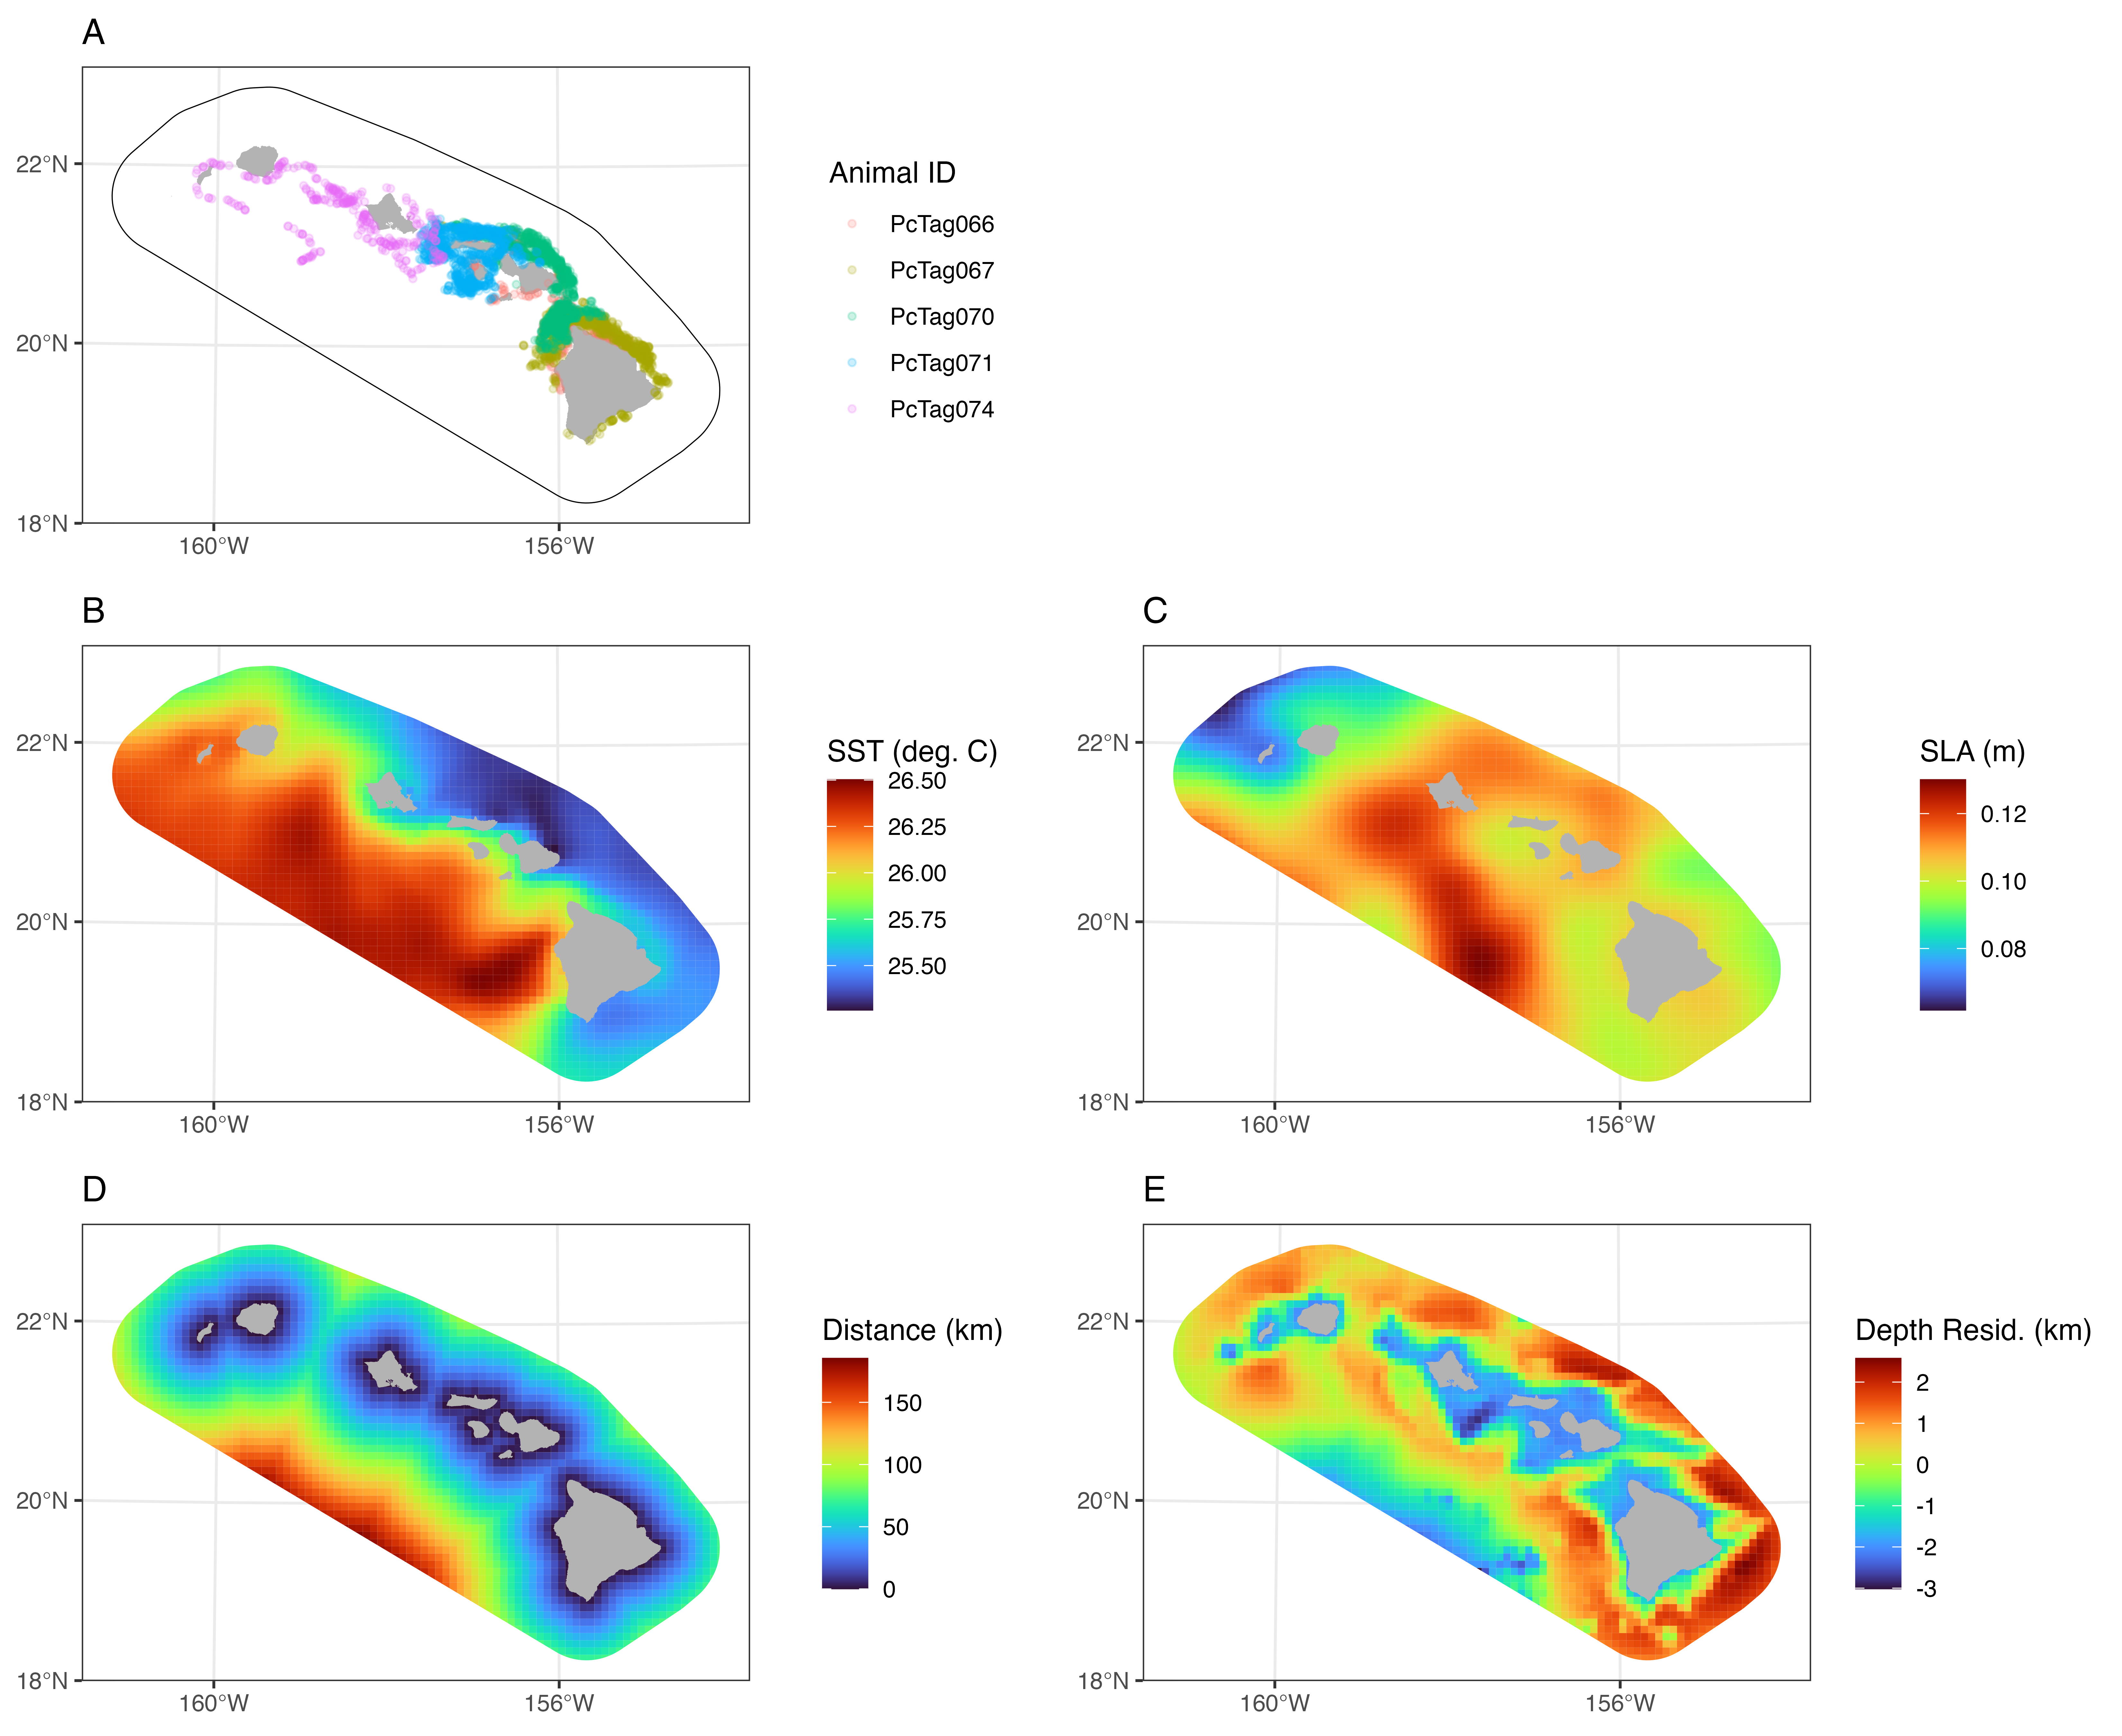
\includegraphics[width=0.75\paperwidth]{figures/data_fig.png}
\caption{\label{fig.data}}
\end{center}
\end{figure}

\clearpage

\begin{figure}
\begin{center}
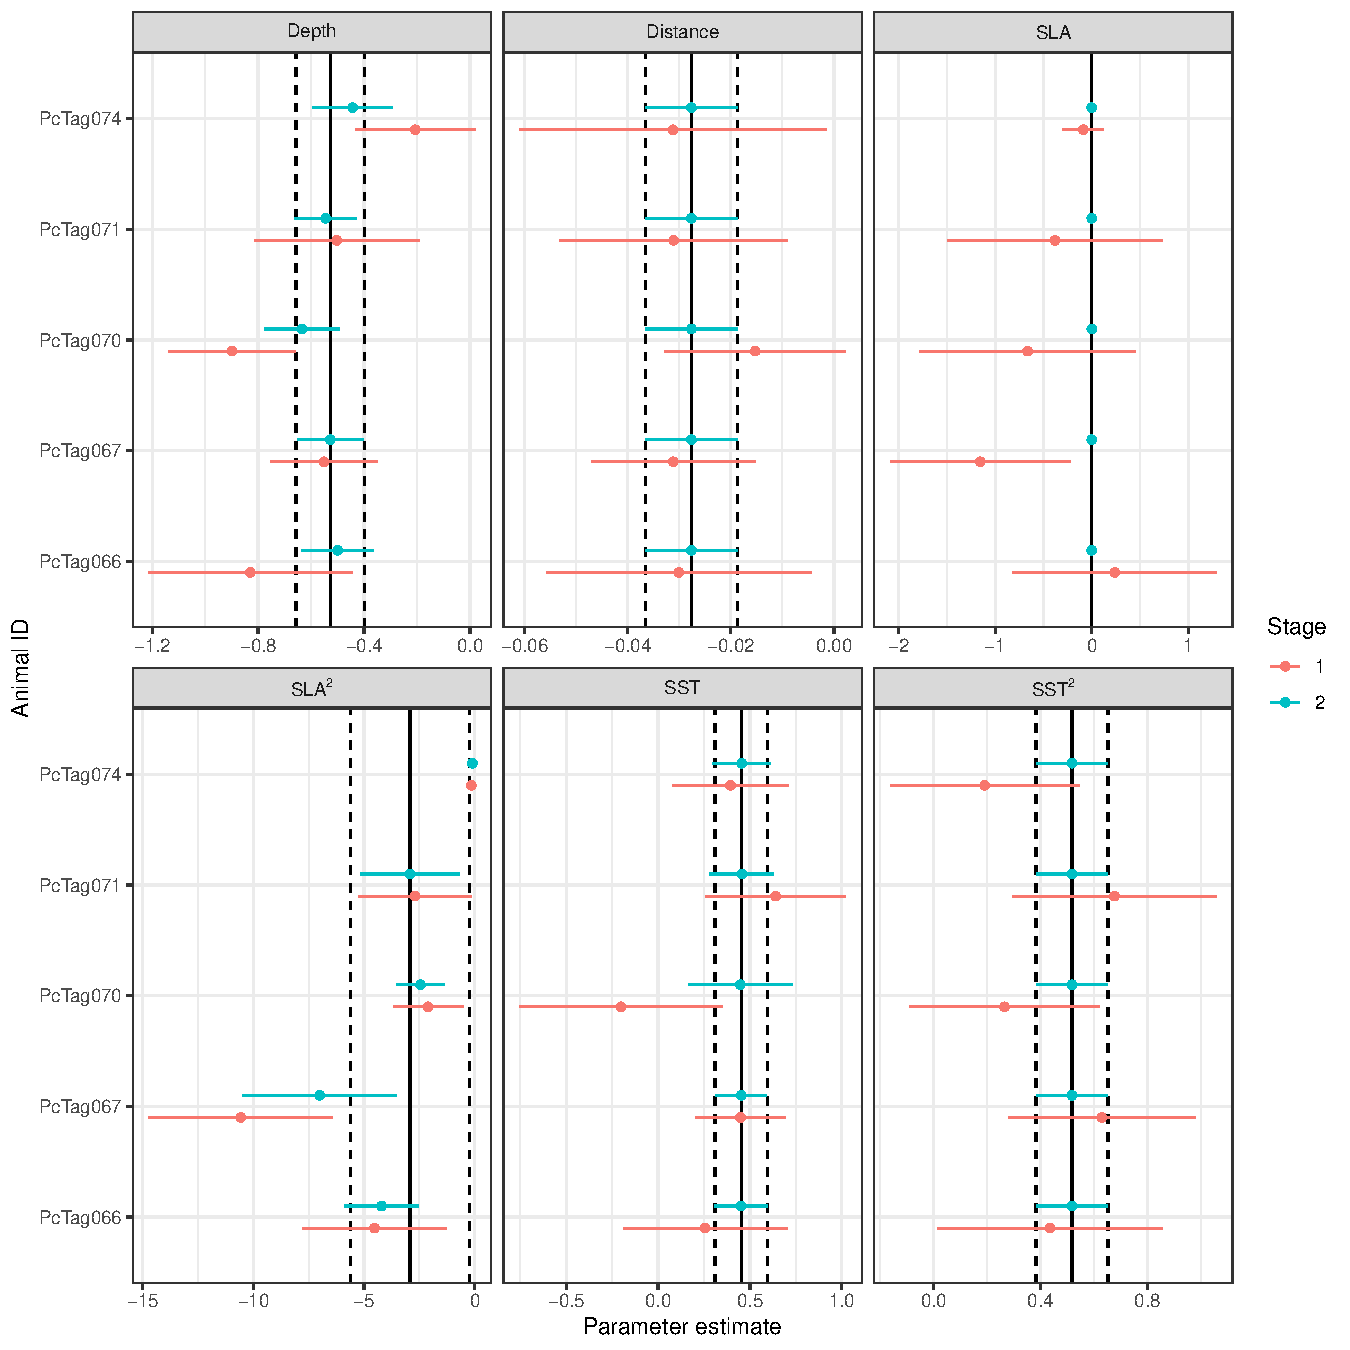
\includegraphics[width=0.75\paperwidth]{figures/par_plt.pdf}
\caption{} 
\end{center}
\end{figure}


\clearpage

\begin{figure}
\begin{center}
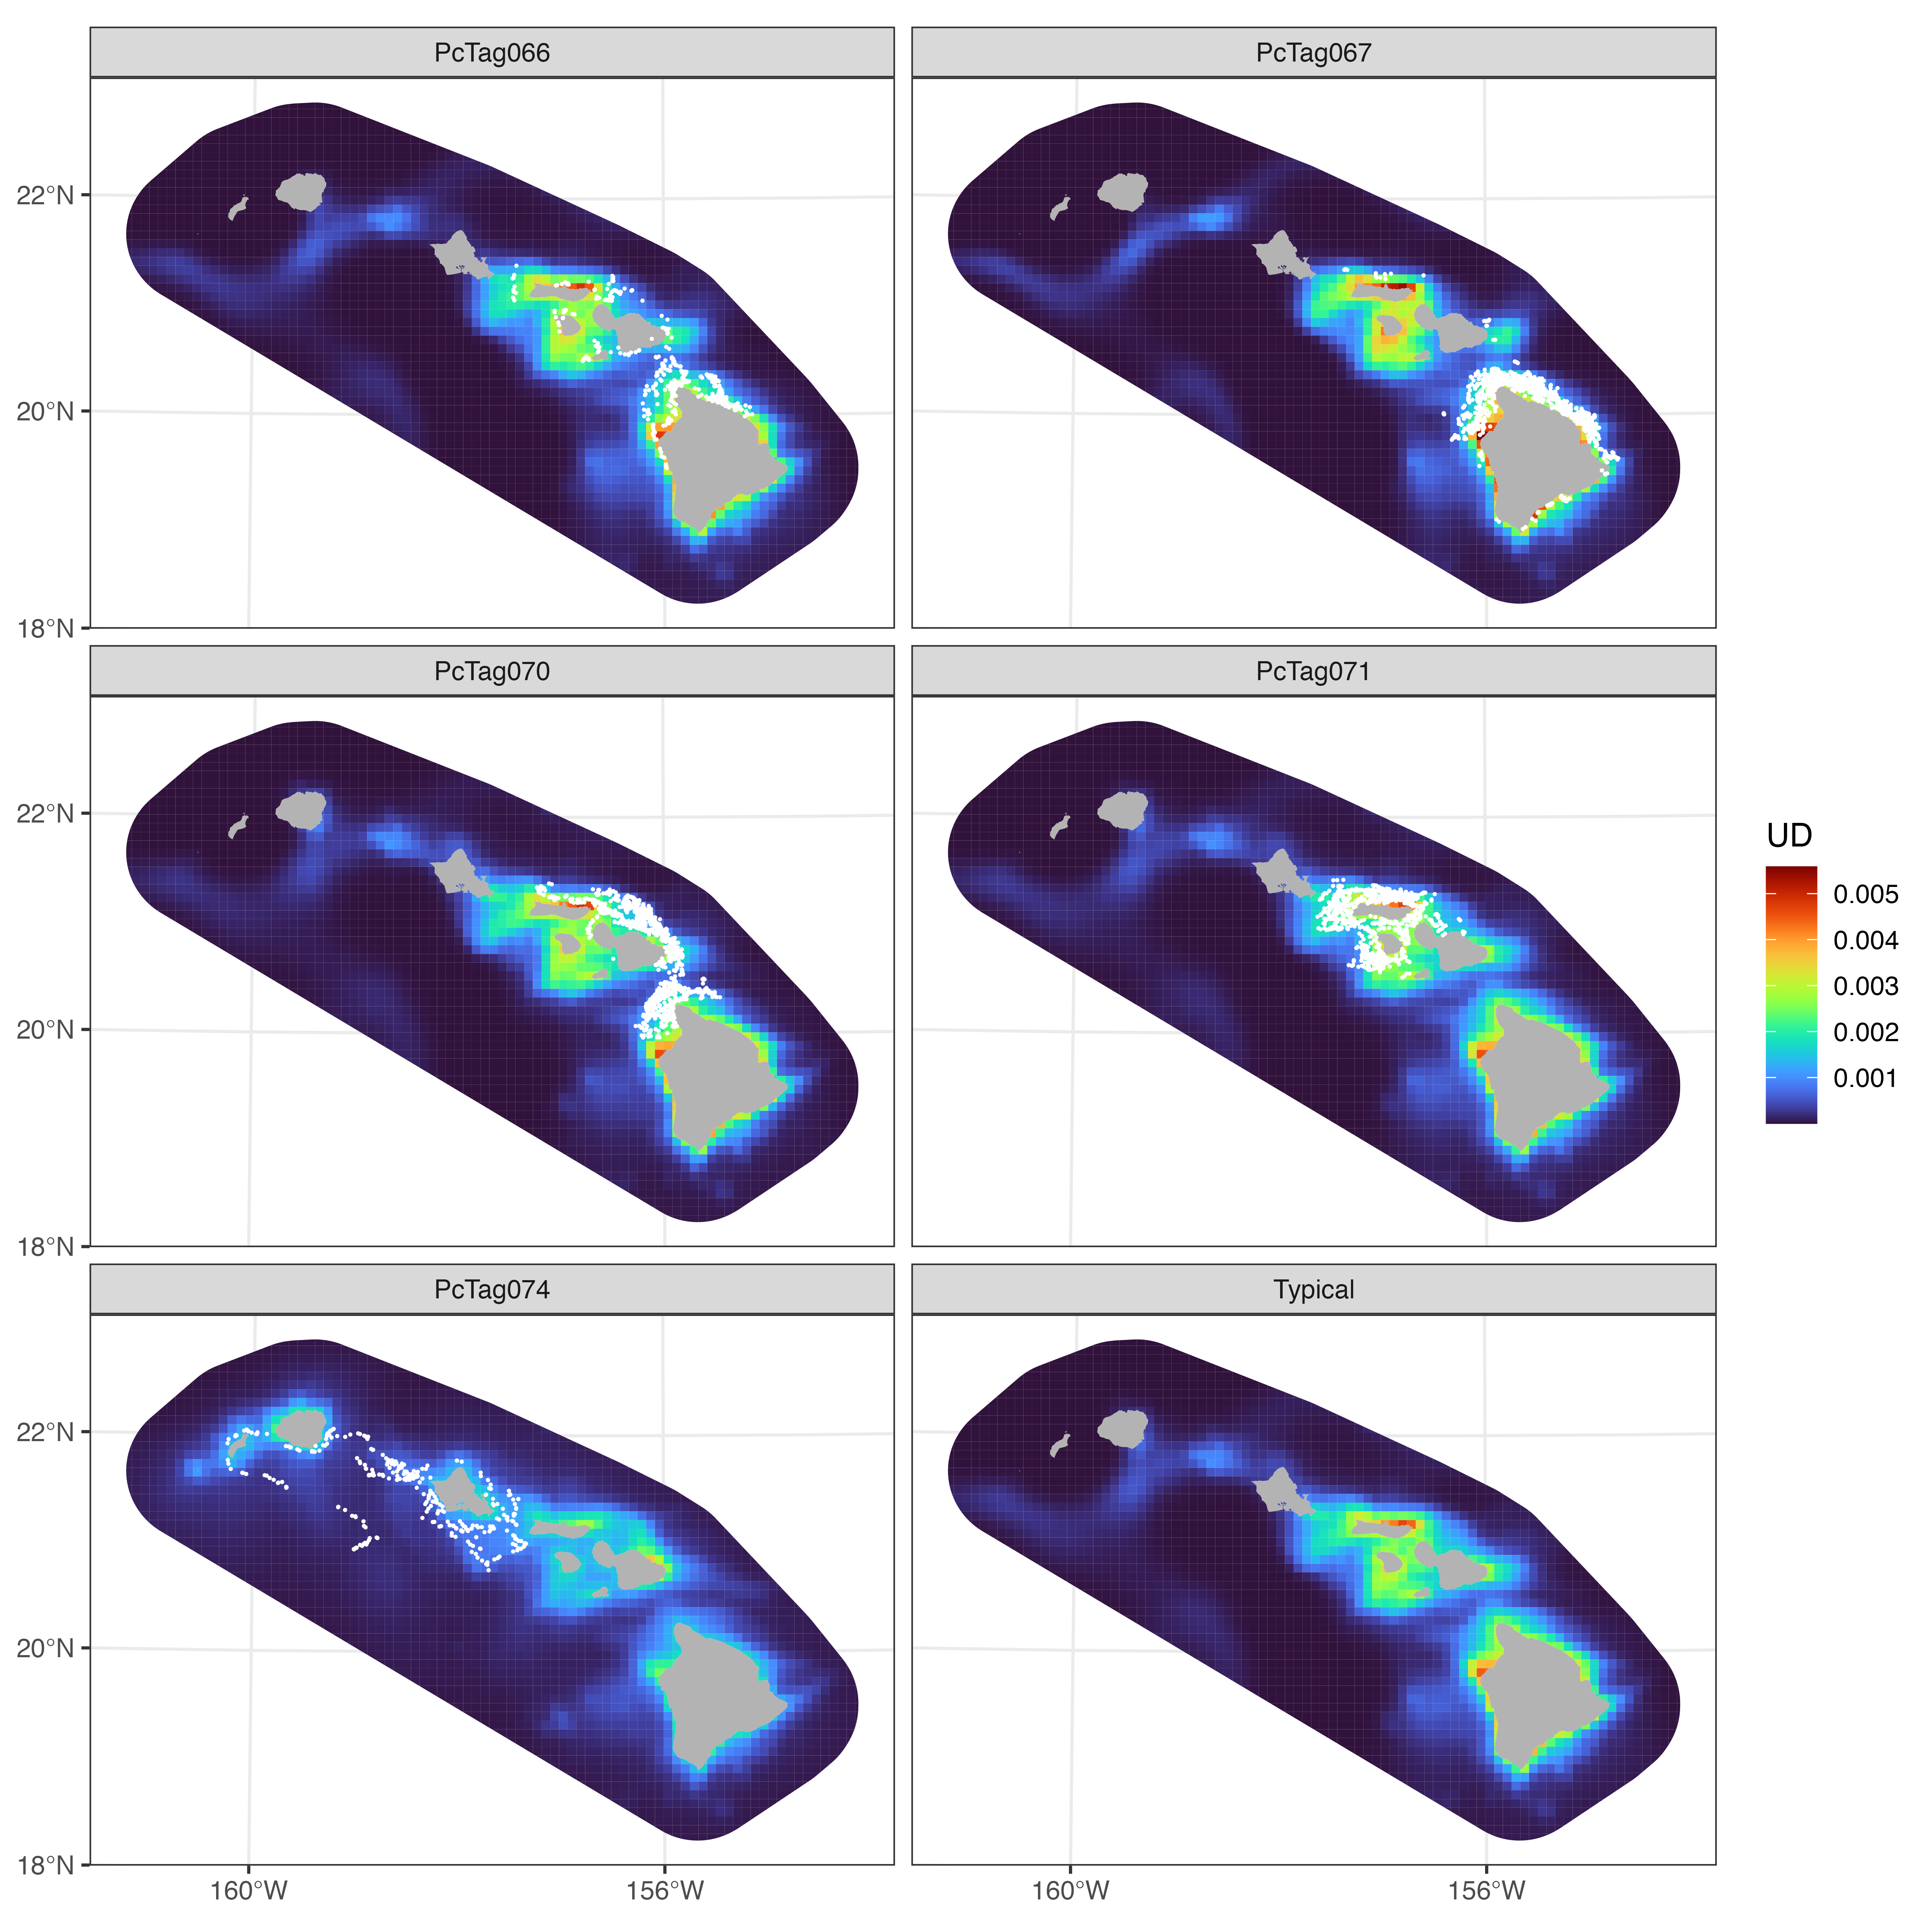
\includegraphics[width=0.75\paperwidth]{figures/meta_fig.png}
\caption{} 
\end{center}
\end{figure}



\end{document}